\begin{enumerate}
	\item In an equilateral $\triangle$ ABC, D is a point on side BC such that $ BD =\frac{1}{3}BC$. Prove that $9(AD)^2 = 7(AB)^2$.
	\hfill\brak{10, 2018}\item Prove that, in a right triangle, the  square on the hypotenuse is equal to sum of the squares on the other two sides.
	\hfill\brak{10, 2018}\item Prove that the area of an equilateral triangle described on one side of the square is equal to half of the area of the equilateral triangle described on one of its diagonal.
	\hfill\brak{10, 2018}\item If the area of two similar triangles are equal, prove that they are congruent.
\hfill\brak{10, 2018}
\item In figure,\figref{fig:rightangled4} BN and CM are medians of a $\triangle$ ABC right-angled at A. Prove that \begin{align}4(BN^2 +CM^2) = 5BC^2\end{align} 
\begin{figure}[!ht]
\centering
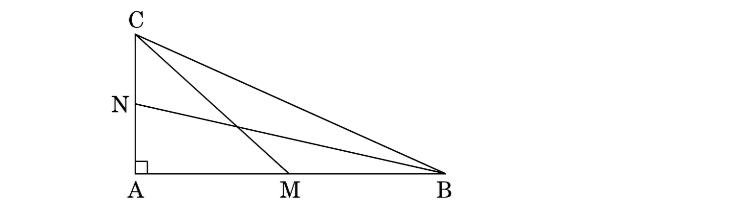
\includegraphics[width=\columnwidth]{cbse/figs/rightangled}
\caption{Right-angled triangle}
\label{fig:rightangled4}
\end{figure}

\hfill\brak{10, 2022}\item If $A$, $B$ and $C$ are interior angles of $ \triangle ABC$, then show that
	\begin{align}
	    \cos \brak{\frac{B + C}{2}}=\sin \brak{\frac{A}{2}}
	\end{align}
      
\hfill\brak{10, 2020} \item Two angles of a triangle are $\cot^{-1}2$ and $\cot^{-1}3$. The third angle of the triangle is?
    
    \hfill\brak{10, 2022}\item  In $\triangle ABC$, right-angled at $A$, if $AB=7 cm$ and $AC=24 cm$, then find $\sin B$
and $\tan C$.

\hfill\brak{10, 2021}\item Two angles of a triangle are  $\cot^{-1}2$ and $\cot^{-1}3$.The third angle of the
triangle is \rule{30pt}{1pt}

\hfill\brak{12, 2021}

\item $A$, $B$ and $C$ are interior angles of a triangle $ABC$. Show that
\begin{enumerate}
\item  $\sin$ $ \brak{{\frac {B+C}{2}}} = \cos {\frac {A}{2}}$
\item  If $\angle A = 90 \degree$ , then find the value of $\tan \brak{{\frac{B+C}{2}}}$ 
\end{enumerate} 

\hfill\brak{10, 2019}	\item In $\triangle$ $ABC$, $AB = {4\sqrt{3}}$ cm, $AC = 8 cm$ and $BC = 4 cm$. The angle $B$ is
				\begin{enumerate}
\item $120\degree$
\item $90\degree$
\item $60\degree$
\item $45\degree$
				\end{enumerate}
	\hfill\brak{10, 2021}

\end{enumerate}
